\section{Fazit}
\label{sec:Fazit}
Im Fazit sollen die technische Implementierung der Software wie auch die Erfüllung der ursprünglichen Zielsetzung in Bezug zu den definierten Anforderungen analysiert und bewertet werden. Dabei werden die Projektphasen, die eingesetzten Technologien, die Qualität der Codebasis sowie die erreichten Funktionalitäten betrachtet. Des Weiteren werden etwaige Herausforderungen und Hindernisse während der Entwicklungsphase beleuchtet und mögliche Gründe für Abweichungen von der ursprünglichen Planung untersucht. Abschließend werden Empfehlungen zur Optimierung und Weiterentwicklung der Software formuliert.

\subsection{Zusammenfassung des Projektes}
\label{sec:Zusammenfassung}
Diese Arbeit widmete sich der Entwicklung eines neuen Anwesenheitsplaners für das SMK mit dem Ziel, die Probleme der bestehenden Lösung mit Excel zu beheben. Bei der Umsetzung wurde sich an den klassischen Phasen eines Softwareentwicklungsprojektes orientiert. Zuerst wurden die Probleme der bestehenden Lösung untersucht. Darauf folgend wurden mithilfe einer Anforderungsanalyse die funktionalen und nichtfunktionalen Soll-Kriterien erhoben. Nach der Analyse wurde eine ausführliche Variantendiskussion durchgeführt die sowohl die Akquisition von Standartsoftware als auch eine Eigenentwicklung in Betracht zog.

Es wurde sich für eine Eigenentwicklung entschieden, da keines der verglichenen Softwareprodukte passend war. Für die Eigenentwicklung wurden dann verschiedene Umsetzungsvarianten wie WebApps und Desktopanwendungen in Betracht gezogen. Am Ende wurde sich für die Entwicklung einer WebApp mit einer Monolith-Systemarchitektur entschieden. Als Framework für die Entwicklung wird Blazor Server eingesetzt.

Nach der Entscheidung für eine Umsetzungsvariante konnte auf Grundlage der Analyse dann der Software- und Systementwurf erstellt werden. Für den Entwurf der Geschäftslogik wurden Ablaufpläne und Klassendiagramme erstellt. Das System soll am Ende aus einem Webserver, der die WebApp hostet und einer Datenbank bestehen. Die Datenbank ist nur mit dem IIS Webserver verbunden und die Clients greifen ausschließlich auf den Webserver zu. Für die Erstellung der Datenbank wurde ein ERM angelegt auf Grundlage der Referenztabelle, siehe Abbildung \ref{abb:Ausgangstabelle} im Anhang.

In der letzten Phase wurden der Entwurf implementiert. Dazu wurde die Datenstruktur in der Datenbank angelegt und die WebApp in Visual Studio entwickelt. Es konnten erfolgreich alle funktionalen Anforderungen implementiert werden, jedoch musste dafür bei der Datenlogik und der Implementierung des MVVM Modells technische Schuld aufgebaut werden. Am Ende konnte der entwickelte Prototyp von mehreren Mitarbeitern getestet werden. Dabei wurde sichtbar, dass der Abbau der technischen Schuld vor der Migration ins Live System notwendig ist, Datenschutz- und Datensicherheit gewährleistet werden müssen. Dementsprechend wird es eine zweite Entwicklungsphase geben müssen, in der die Fehler behoben werden sollen.

\subsection{Vorstellung des Prototypen}
\label{sec:Prototyp}
Als Ergebnis des Projektes konnte ein funktionsfähiger Prototyp entwickelt werden. Dieser ermöglicht es den Benutzern mit Single Sign-on auf die Weboberfläche des Anwesenheitsplaners zuzugreifen und dadurch die Anwesenheitsdaten zu verwalten. Die Benutzeroberfläche konnte sehr intuitiv gestaltet werden, was im Testverfahren mit den Mitarbeitern als sehr positiv aufgefasst wurde. Die gesamte Benutzeroberfläche des Prototypen ist in Abbildung \ref{abb:Prototyp} im Anhang einsehbar.

\begin{figure}[htb]
    \centering
    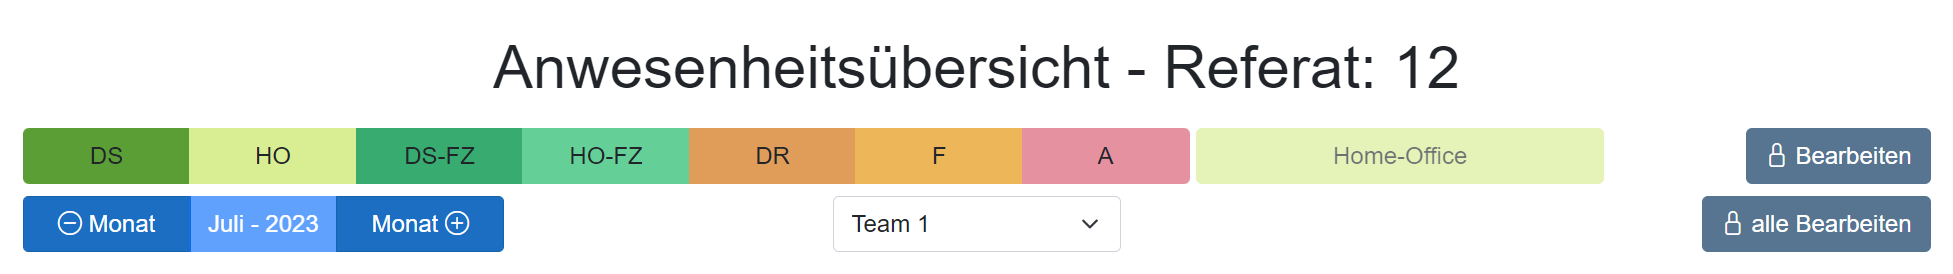
\includegraphics[width=1\textwidth,angle=0]{abb/Buttons_GUI.png}
    \caption[Schaltflächen]{Schaltflächen}
    \label{abb:Buttons_GUI}
\end{figure}

Die Interaktion findet hauptsächlich über die Schaltflächen der Tabelle statt. Dort wird der gewünschte Anwesenheitsstatus ausgewählt, welcher anschließend durch das Klicken auf die Tabellenzelle für diesen Tag gesetzt wird. Die Schaltflächenübersicht ist in Abbildung \ref{abb:Buttons_GUI} zu sehen. Über die Schaltflächen \textit{Bearbeiten} und \textit{alle Bearbeiten} kann zwischen den Lese- \bzw Schreibmodus gewechselt werden. Dabei ist die Schaltfläche \textit{alle Bearbeiten} nur für Konten in der AD Gruppe AWPadmin mit einer Funktion hinterlegt.

Die Monatsansichten, links in blau, zeigen in der Mitte den aktuellen Monat und lassen sich mit den Schaltfläche links und rechts der Mitte um je einen Monat verschieben. Als letzte Schaltfläche kann der aktuell angemeldete Benutzer eine Teamzugehörigkeit auswählen, wodurch sich die Sortierung in der angezeigten Tabelle ändert. Damit können referatsinterne Substrukturen in dem Anwesenheitsplaner abgebildet werden.

Weitere Funktionen sind in Abbildung \ref{abb:Prototyp} im Anhang zu sehen. So sind \zB Feiertage und Wochenenden mit Gelb markiert und können keinen Anwesenheitsstatus bekommen. Der aktuelle Tag ist rot markiert wie im Falle der Abbildung der 18.07.2023.

\subsection{Soll-Ist-Vergleich}
\label{sec:Soll-Ist-Vergleich}
Der Soll-Ist-Vergleich zeigt, dass nahezu alle geplanten Funktionalitäten problemlos umgesetzt wurden. Die in der Use-Case-Analyse definierten funktionalen Anforderungen an das System wurden zufriedenstellend erfüllt. Das ist auf eine gute Analysephase zurückzuführen, da die Referenztabelle eine gute Vorlage für die zu entwickelnde Software bot. Allerdings haben die umfangreichen Tests auch einige Schwachstellen aufgezeigt. Insbesondere die Systemsicherheit und der Datenschutz müssen noch weiter ausgebaut werden, um den Prototypen auf den Einsatz in der produktiven Umgebungen vorzubereiten. Insbesondere ein Datenschutzkonzept, welches Aufbewahrungsfristen und den Umgang auf die Anwesenheitsdaten regelt, muss von der Datenschutzbeauftrageten im SMK abgesegnet werden. Auch müssen im Bereich der Datensicherheit noch Nachbesserungen erfolgen. Ein Kritikpunk stellt \zB das fehlende Logging in der WebApp dar. Zwar werden  standardmäßig vom Webserver und von der Datenbank Logs erzeugt, doch wird ein spezifisches Logging der Geschäftslogik gefordert. Ein weiter Punkt ist das alle Eingaben sowohl im Frontend als auch im Backend validiert werden, um Fehler zu minimieren und mögliche Angriffsvektoren zu schließen.

Abschließend ist zu sagen, dass der funktionale Soll-Zustand erreicht werden konnte, aber nur durch Abstriche in Codequalität und Sicherheitsfeatures, was auf den knapp bemessenen Zeitrahmen sowie fehlende Kenntnisse zurückzuführen ist.

\subsection{Bewertung der Umsetzung des Projektes}
\label{sec:Bewertung} %werden die Projektphasen,eingesetzten Technologien, die Qualität der Codebasis,Herausforderungen und Hindernisse während der Entwicklungsphase, Abweichungen von der ursprünglichen Planung
Die Umsetzung des Projektes verlief insgesamt erfolgreich, da durch eine solide Planung ein klarer Ablauf des Projektes definierte wurde. Dabei gab es in der Planung und Analyse keine nennenswerten Schwierigkeiten. Das änderte sich bei der Phase der Variantendiskussion, da keinerlei Vorwissen zu den Themen System- und Softwarearchitekturen vorhanden waren. Dies erschwerte den Prozess der Auswahl einer Umsetzungsvariante erheblich, da in der Folge das Wissen erst aufgebaut werden musste.

Die Auswahl der Technologien für die Umsetzung erwies sich im Nachhinein als sehr gelungen, sodass mit nur geringem Aufwand die benötigten Funktionalitäten realisiert werden konnten. Das gründete sich vor allem Dingen in der Wahl des Csharp basierten Blazor Server Frameworks. Dadurch konnte das vorhandene Csharp Vorwissen verwendet werden und ohne die Nutzung von Javascript eine funktionsfähige Weboberfläche erstellt werden. Nachteilig am Einsatz des Frameworks war die geplante Anwendung des MVVM Musters für die Benutzerinteraktionen. Durch den Aufbau einer Razor Page muss das MVVM Muster anders als bei vorher verwendeten Frameworks implementiert werden. Das führte dazu, dass das Muster nicht sauber implementiert werden konnte. Es resultierte eine zu niedrige Qualität der Codebasis, was schließlich in der zweiten Entwicklungsphase angegangen werden sollte.

Die größten Schwierigkeiten lagen in der Umsetzung der Datenschutz- und Datensicherheitsrichtlinien. Hier gab es während der Analyse-, Entwurf- und Implementierungs-Phase immer wieder Rücksprachen mit den verantwortlichen im SMK. Doch angemessene Maßnahmen für die geforderten Standards des BSI zu finden und diese Umzusetzen gestalten, stellte sich als viel zeitintensiver heraus, als erwartet. Deswegen musste von dem Plan ein für den Einsatz im Live System geeignete Software zu entwickeln Abstand genommen werden. Stattdessen wurde die Software als Prototyp zur Demonstration sowie für Tests verwendet, welche in einer zweiten Entwicklungsphase weiter angepasst werden sollen.

\newpage
\subsection{Ausblick}
\label{sec:Ausblick}

Der Prototyp erfüllt bereits viele der gestellten Anforderungen und zeigt großes Potenzial zur Verbesserung des aktuellen Prozesses an. Allerdings bedarf es noch weiterer Arbeit, um die noch bestehenden Mängel zu beheben und das System für den produktiven Einsatz vorzubereiten.

Die zweite Entwicklungsphase wird daher darauf ausgerichtet werden, die technische Schuld abzubauen, Datenschutz- und Datensicherheitsmaßnahmen zu implementieren und das System um Schnittstellen und Funktionen zu erweitern. Die anhaltende enge Zusammenarbeit mit den Referaten im SMK bleibt in diesem Prozess von zentraler Bedeutung. Die Wünsche und Rückmeldungen werden berücksichtigt und eingearbeitet, sodass ein optimaler Lösungsvorgang stattfinden kann. Während der Präsentation des Prototypen konnten bereits viele Wünsche und Anmerkungen in Bezug zu erweiterten Funktionalitäten erfasst werden. Diese wurden notiert und für die nächste Entwicklungsphase vermerkt. In Zukunft soll wiederholt Zeit in die Weiterentwicklung des Anwesenheitsplaner investiert werden, sodass dieser so bald wie möglich für die Migration bereitsteht.

\subsection{Schlusswort}
\label{sec:Abschluss}

Abschließend wird festgehalten, dass die Entwicklung des Anwesenheitsplaners ein herausforderndes, aber zugleich äußerst interessantes Projekt darstellte. Die gewonnenen Erkenntnisse und Erfahrungen werden für zukünftige Entwicklungsprojekte von großem Nutzen sein. Der größtmögliche Lernfortschritt konnte während der Recherche zu den System- und Softwarearchitekturen erzielt werden. In dieser ersten Auseinandersetzung mit der Thematik konnten neue Kompetenzen gewonnen werden, die zukünftig weiterhin ausgebaut und angewandt werden sollen.

